%%%%%%%%%%%%%%%%%%%%%%%%%%%%%%%%%%%%%%%%%
% Short Sectioned Assignment
% LaTeX Template
% Version 1.0 (5/5/12)
%
% This template has been downloaded from:
% http://www.LaTeXTemplates.com
%
% Original author:
% Frits Wenneker (http://www.howtotex.com)
%
% License:
% CC BY-NC-SA 3.0 (http://creativecommons.org/licenses/by-nc-sa/3.0/)
%
%%%%%%%%%%%%%%%%%%%%%%%%%%%%%%%%%%%%%%%%%

%----------------------------------------------------------------------------------------
%	PACKAGES AND OTHER DOCUMENT CONFIGURATIONS
%----------------------------------------------------------------------------------------

\documentclass[paper=a4, fontsize=11pt]{scrartcl} % A4 paper and 11pt font size

\usepackage[T1]{fontenc} % Use 8-bit encoding that has 256 glyphs
%\usepackage{fourier} % Use the Adobe Utopia font for the document - comment this line to return to the LaTeX default
\usepackage[english]{babel} % English language/hyphenation
\usepackage[utf8]{inputenc}  %allows non-English characters
\usepackage{amsmath,amsfonts,amsthm} % Math packages

\usepackage{sectsty} % Allows customizing section commands
%\allsectionsfont{\centering \normalfont\scshape} % Make all sections centered, the default font and small caps
\allsectionsfont{\centering}

\usepackage{fancyhdr} % Custom headers and footers
\pagestyle{fancyplain} % Makes all pages in the document conform to the custom headers and footers
\fancyhead{} % No page header - if you want one, create it in the same way as the footers below
\fancyfoot[L]{} % Empty left footer
\fancyfoot[C]{} % Empty center footer
\fancyfoot[R]{\thepage} % Page numbering for right footer
\renewcommand{\headrulewidth}{0pt} % Remove header underlines
\renewcommand{\footrulewidth}{0pt} % Remove footer underlines
\setlength{\headheight}{13.6pt} % Customize the height of the header

%\usepackage{geometry}
%\usepackage{pdflscape}


%\numberwithin{equation}{section} % Number equations within sections (i.e. 1.1, 1.2, 2.1, 2.2 instead of 1, 2, 3, 4)
%\numberwithin{figure}{section} % Number figures within sections (i.e. 1.1, 1.2, 2.1, 2.2 instead of 1, 2, 3, 4)
%\numberwithin{table}{section} % Number tables within sections (i.e. 1.1, 1.2, 2.1, 2.2 instead of 1, 2, 3, 4)

%\setlength\parindent{0pt} % Removes all indentation from paragraphs - comment this line for an assignment with lots of text

\usepackage{caption}
%\usepackage{topcapt}

\usepackage{booktabs}

\usepackage{graphicx}
\usepackage{adjustbox}
\graphicspath{{../images/}}


%shortcuts for typing variance and expectation 
\newcommand{\E}{\mathrm{E}}
\newcommand{\Var}{\mathrm{Var}}

%----------------------------------------------------------------------------------------
%	TITLE SECTION
%----------------------------------------------------------------------------------------

\newcommand{\horrule}[1]{\rule{\linewidth}{#1}} % Create horizontal rule command with 1 argument of height

\title{	
\normalfont \normalsize 
\textsc{UPC - Complex and Social Networks} \\ [25pt] % Your university, school and/or department name(s)
\horrule{0.5pt} \\[0.4cm] % Thin top horizontal rule
\huge Lab4: Non-linear regression on dependency trees \\ % The assignment title
\horrule{2pt} \\[0.5cm] % Thick bottom horizontal rule
}

\author{Paul\\Simon Van den Eynde} % Your name

\date{\normalsize\today} % Today's date or a custom date

\begin{document}


\maketitle % Print the title


%----------------------------------------------------------------------------------------
%	INTRO
%----------------------------------------------------------------------------------------

\section{Introduction}

%----------------------------------------------------------------------------------------
%	Results
%----------------------------------------------------------------------------------------
\section{Results}
%----------------------------------------------------------------------------------------
%	Tables
%----------------------------------------------------------------------------------------
\begin{table}
\begin{adjustbox}{center}
\centering
\begin{tabular}{rrrrrrrrrrrr}
  Language & 0 & 1 & 2 & 3 & 1+ & 2+ & 3+ & 4 & 4+ & 5 & 5+ \\ 
  \midrule
Arabic & 9.52 & 0.66 & 0.66 & 0.72 & 0.66 & 0.66 & 0.66 & 0.68 & 0.68 & 0.65 & 0.66 \\ 
  Basque & 2.75 & 0.45 & 0.45 & 0.49 & 0.45 & 0.45 & 0.45 & 0.46 & 0.46 & 0.45 & 0.45 \\ 
  Catalan & 7.73 & 0.53 & 0.53 & 0.55 & 0.53 & 0.53 & 0.53 & 0.53 & 0.53 & 0.53 & 0.53 \\ 
  Chinese & 1.28 & 0.35 & 0.34 & 0.36 & 0.34 & 0.34 & 0.34 & 0.37 & 0.35 & 0.34 & 0.34 \\ 
  Czech & 4.86 & 0.65 & 0.64 & 0.68 & 0.94 & 0.64 & 0.64 & 0.67 & 0.66 & 0.63 & 0.63 \\ 
  English & 6.22 & 0.70 & 0.69 & 0.72 & 0.69 & 0.69 & 0.69 & 0.69 & 0.69 & 0.69 & 0.69 \\ 
  Greek & 7.16 & 0.57 & 0.57 & 0.62 & 0.57 & 0.57 & 0.57 & 0.58 & 0.58 & 0.57 & 0.57 \\ 
  Hungarian & 4.75 & 1.09 & 1.09 & 1.20 & 1.09 & 1.10 & 1.09 & 1.25 & 1.15 & 1.09 & 1.09 \\ 
  Italian & 5.98 & 0.53 & 0.53 & 0.58 & 0.53 & 0.52 & 0.53 & 0.54 & 0.54 & 0.53 & 0.53 \\ 
  Turkish & 3.13 & 0.55 & 0.55 & 0.60 & 0.54 & 0.55 & 0.54 & 0.56 & 0.56 & 0.54 & 0.54 \\ 
   \bottomrule
\end{tabular}
\end{adjustbox}
\caption{Residual standard error for every model and language}
\label{tab:s}
\end{table}

% latex table generated in R 3.1.2 by xtable 1.7-4 package
% Thu Nov 10 12:54:07 2016
\begin{table}
\begin{adjustbox}{center}
\centering
\begin{tabular}{rrrrrrrrrrrr}
 Language & 0 & 1 & 2 & 3 & 1+ & 2+ & 3+ & 4 & 4+ & 5 & 5+ \\ 
  \midrule
Arabic & 30174 & 8238 & 8217 & 9013 & 8220 & 8207 & 8278 & 8535 & 8439 & 8183 & 8221 \\ 
  Basque & 14267 & 3608 & 3581 & 4112 & 3584 & 3582 & 3590 & 3738 & 3733 & 3583 & 3585 \\ 
  Catalan & 104292 & 23473 & 23406 & 24856 & 23358 & 23480 & 23462 & 23593 & 23595 & 23433 & 23435 \\ 
  Chinese & 180870 & 40240 & 38009 & 44305 & 38436 & 37332 & 37258 & 44946 & 40632 & 37921 & 37781 \\ 
  Czech & 150242 & 49676 & 49033 & 51950 & 68101 & 48876 & 48759 & 50654 & 50616 & 48049 & 48270 \\ 
  English & 121969 & 39929 & 39448 & 41178 & 39315 & 39364 & 39420 & 39323 & 39276 & 39287 & 39367 \\ 
  Greek & 19992 & 5096 & 5070 & 5550 & 5071 & 5083 & 5096 & 5202 & 5199 & 5073 & 5075 \\ 
  Hungarian & 38251 & 19382 & 19367 & 20608 & 19380 & 19407 & 19388 & 21121 & 20009 & 19370 & 19372 \\ 
  Italian & 26584 & 6511 & 6451 & 7252 & 6438 & 6423 & 6489 & 6677 & 6652 & 6428 & 6430 \\ 
  Turkish & 30859 & 9937 & 9810 & 10901 & 9759 & 9799 & 9722 & 10116 & 10111 & 9794 & 9784 \\ 
   \bottomrule
\end{tabular}
\end{adjustbox}
\caption{AIC for every model and language}
\label{tab:aic}
\end{table}


% latex table generated in R 3.1.2 by xtable 1.7-4 package
% Thu Nov 10 12:54:37 2016
\begin{table}
\begin{adjustbox}{center}
\centering
\begin{tabular}{rrrrrrrrrrrr}
 Language & 0 & 1 & 2 & 3 & 1+ & 2+ & 3+ & 4 & 4+ & 5 & 5+ \\ 
  \midrule
Arabic & 21991.4 & 55.0 & 34.7 & 830.4 & 37.0 & 24.3 & 95.7 & 352.2 & 255.8 & 0.0 & 37.7 \\ 
  Basque & 10685.9 & 27.6 & 0.0 & 531.3 & 3.0 & 0.8 & 8.7 & 157.3 & 152.0 & 1.9 & 3.9 \\ 
  Catalan & 80934.9 & 115.8 & 48.5 & 1498.2 & 0.0 & 122.1 & 104.3 & 235.7 & 237.4 & 75.5 & 77.5 \\ 
  Chinese & 143612.3 & 2982.4 & 750.8 & 7046.6 & 1178.0 & 73.6 & 0.0 & 7688.2 & 3373.6 & 662.6 & 522.9 \\ 
  Czech & 102192.8 & 1627.0 & 983.2 & 3900.6 & 20051.5 & 827.1 & 710.0 & 2604.2 & 2567.0 & 0.0 & 220.5 \\ 
  English & 82693.4 & 653.3 & 172.4 & 1901.9 & 39.2 & 88.4 & 144.3 & 47.2 & 0.0 & 11.4 & 91.2 \\ 
  Greek & 14921.4 & 25.3 & 0.0 & 479.9 & 1.1 & 12.9 & 26.0 & 131.6 & 129.0 & 2.4 & 4.4 \\ 
  Hungarian & 18883.8 & 14.4 & 0.0 & 1241.0 & 12.7 & 39.4 & 20.8 & 1753.7 & 641.3 & 2.6 & 4.6 \\ 
  Italian & 20160.4 & 87.4 & 27.9 & 828.8 & 14.4 & 0.0 & 65.1 & 253.6 & 228.8 & 4.6 & 6.6 \\ 
  Turkish & 21137.2 & 214.9 & 88.5 & 1179.0 & 37.4 & 77.2 & 0.0 & 393.5 & 389.1 & 72.3 & 61.6 \\ 
   \bottomrule
\end{tabular}
\end{adjustbox}
\caption{Difference in AIC with best model for every language}
\label{tab:daic}
\end{table}

% latex table generated in R 3.1.2 by xtable 1.7-4 package
% Thu Nov 10 13:05:51 2016
\begin{table}[ht]
\centering
\begin{tabular}{rrrrrr}
  Language & N & $\mu_{n}$ & $\sigma_{n}$ & $\mu_{x}$ & $\sigma_{x}$ \\ 
  \midrule
Arabic & 4108 & 27 & 20.6 & 2.17 & 0.93 \\ 
  Basque & 2933 & 11 & 6.5 & 1.96 & 0.69 \\ 
  Catalan & 15053 & 26 & 13.6 & 2.32 & 0.70 \\ 
  Chinese & 54238 & 6 & 3.3 & 1.44 & 0.48 \\ 
  Czech & 25037 & 16 & 10.7 & 2.02 & 0.87 \\ 
  English & 18779 & 24 & 11.2 & 3.05 & 0.90 \\ 
  Greek & 2951 & 23 & 14.4 & 2.20 & 0.81 \\ 
  Hungarian & 6424 & 22 & 12.6 & 3.88 & 1.78 \\ 
  Italian & 4144 & 18 & 13.3 & 1.97 & 0.77 \\ 
  Turkish & 6030 & 11 & 8.3 & 1.84 & 0.82 \\ 
   \bottomrule
\end{tabular}
\caption{Basic information}
\label{tab:bi}
\end{table}


% latex table generated in R 3.1.2 by xtable 1.7-4 package
% Thu Nov 10 13:10:37 2016
\begin{table}
\begin{adjustbox}{width=1.4\textwidth,center}
\centering
\begin{tabular}{rrrrrrrrrrrrrrrrrrrrrrrr}
  &\multicolumn{23}{c}{Model}\\
  \cmidrule{2-24}
  Language & 1 & \multicolumn{2}{c}{2} & \multicolumn{2}{c}{3} & \multicolumn{2}{c}{1+} & \multicolumn{3}{c}{2+} & \multicolumn{3}{c}{3+} & 4 & \multicolumn{2}{c}{4+} & \multicolumn{3}{c}{5} & \multicolumn{4}{c}{5+}\\
  \midrule
 & b & a & b & a & c & b & d & a & b & d & a & c & d & a & a & d & a & b & c & a & b & c & d \\ 
  \midrule
Arabic & 0.34 & 0.7 & 0.36 & 1.6 & 0.01 & 0.34 & -0.06 & 0.52 & 0.41 & 0.32 & -3.1 & -0.02 & 4.1 & 0.73 & 0.63 & 0.32 & 0.83 & 0.29 & 0.0021 & 1.1 & 0.22 & 0.0028 & -0.21 \\ 
  Basque & 0.42 & 0.67 & 0.46 & 1.3 & 0.032 & 0.44 & -0.094 & 0.61 & 0.48 & 0.088 & -3.3 & -0.044 &   4 & 0.87 & 0.83 & 0.086 & 0.7 & 0.43 & 0.0022 & 0.7 & 0.43 & 0.0022 & 0 \\ 
  Catalan & 0.35 & 0.72 & 0.37 & 1.7 & 0.012 & 0.35 & -0.025 & 0.87 & 0.33 & -0.15 & -2.6 & -0.03 & 3.6 & 0.75 & 0.75 & 0.012 & 0.8 & 0.32 & 0.0017 & 0.8 & 0.32 & 0.0017 & 0 \\ 
  Chinese & 0.38 & 0.6 & 0.5 & 1.1 & 0.048 & 0.45 & -0.15 & 0.26 & 0.71 & 0.51 & -3.8 & -0.037 & 4.5 & 0.83 & 0.64 & 0.35 & 0.73 & 0.36 & 0.0087 & 0.43 & 0.51 & 0.0048 & 0.33 \\ 
  Czech & 0.36 & 0.62 & 0.44 & 1.5 & 0.016 & -72 &   2 & 0.23 & 0.66 & 0.58 &  19 & 0.0029 & -18 & 0.79 & 0.75 & 0.093 & 0.82 & 0.28 & 0.0085 & 1.1 & 0.21 & 0.01 & -0.22 \\ 
  English & 0.46 & 0.95 & 0.37 & 2.2 & 0.014 & 0.42 & 0.3 & 0.96 & 0.39 & -0.16 & -3.4 & -0.04 & 4.5 &   1 & 1.1 & -0.2 & 0.91 & 0.39 & -0.00091 &  64 & 0.012 & 0.00021 & -64 \\ 
  Greek & 0.35 & 0.71 & 0.38 & 1.6 & 0.014 & 0.36 & -0.1 & 0.57 & 0.41 & 0.18 &  -3 & -0.028 & 3.9 & 0.76 & 0.73 & 0.089 & 0.73 & 0.37 & 0.00045 & 0.73 & 0.37 & 0.00045 & 0 \\ 
  Hungarian & 0.59 & 0.61 & 0.61 & 2.4 & 0.021 & 0.6 & -0.13 & 0.61 & 0.61 & 0.1 & -11 & -0.015 &  12 & 1.4 & 2.1 & -2.3 & 0.59 & 0.63 & -0.00075 & 0.59 & 0.63 & -0.00075 & 0 \\ 
  Italian & 0.35 & 0.63 & 0.41 & 1.5 & 0.015 & 0.36 & -0.13 & 0.46 & 0.46 & 0.32 &  -3 & -0.026 & 3.9 & 0.74 & 0.69 & 0.15 & 0.77 & 0.31 & 0.0034 & 0.77 & 0.31 & 0.0034 & 0 \\ 
  Turkish & 0.41 & 0.69 & 0.43 & 1.3 & 0.029 & 0.44 & -0.16 & 0.55 & 0.49 & 0.2 & -3.7 & -0.036 & 4.4 & 0.85 & 0.88 & -0.061 & 0.63 & 0.5 & -0.0032 & 0.56 & 0.53 & -0.0038 & 0.092 \\ 
   \bottomrule
\end{tabular}
\end{adjustbox}
\caption{Calculated parameters for every model and language}
\label{tab:par}
\end{table}

\newpage
%----------------------------------------------------------------------------------------
%	Best model plots
%----------------------------------------------------------------------------------------
\captionsetup{justification=centering,margin=.2cm}

\begin{figure}
\centering
\begin{minipage}{.5\textwidth}
  \centering
  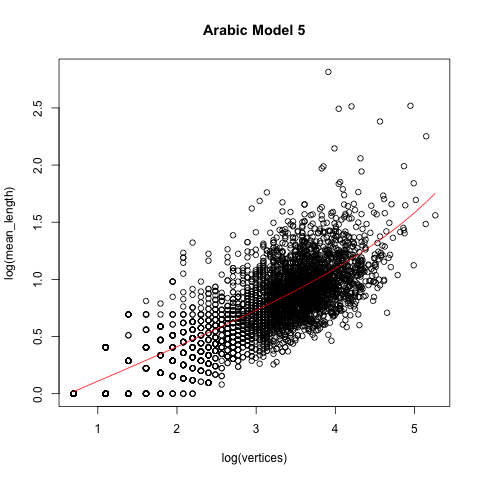
\includegraphics[width=\linewidth]{bestModel_Arabic.png}
  \captionof{figure}{The best model in a log-log plot for Arabic}
  \label{fig:1}
\end{minipage}%
\begin{minipage}{.5\textwidth}
  \centering
  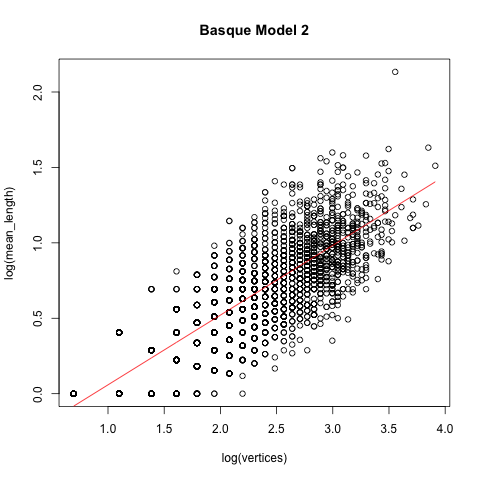
\includegraphics[width=\linewidth]{bestModel_Basque.png}
  \captionof{figure}{The best model in a log-log plot for Basque}
  \label{fig:2}
\end{minipage}
\end{figure}

\begin{figure}
\centering
\begin{minipage}{.5\textwidth}
  \centering
  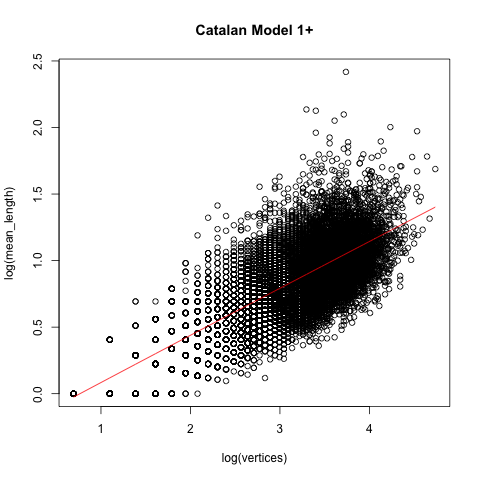
\includegraphics[width=\linewidth]{bestModel_Catalan.png}
  \captionof{figure}{The best model in a log-log plot for Catalan}
  \label{fig:3}
\end{minipage}%
\begin{minipage}{.5\textwidth}
  \centering
  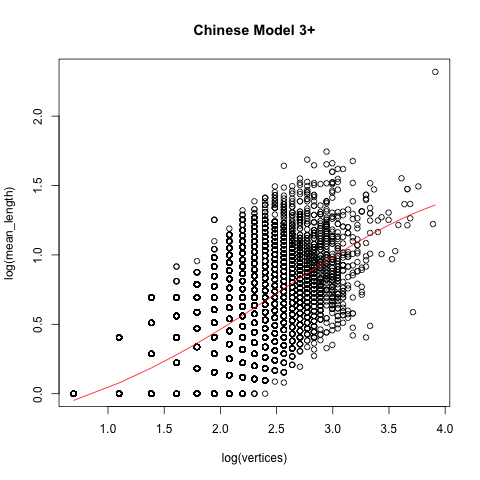
\includegraphics[width=\linewidth]{bestModel_Chinese.png}
  \captionof{figure}{The best model in a log-log plot for Chinese}
  \label{fig:4}
\end{minipage}
\end{figure}

\begin{figure}
\centering
\begin{minipage}{.5\textwidth}
  \centering
  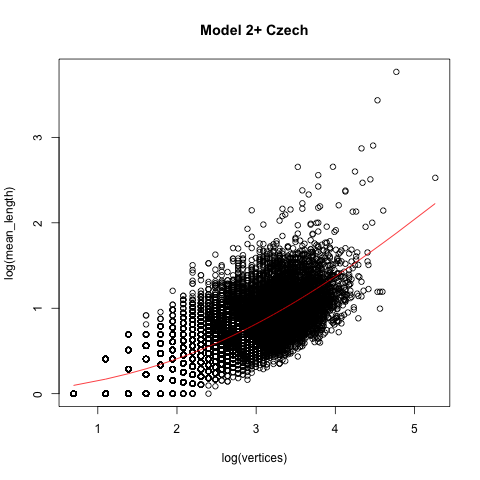
\includegraphics[width=\linewidth]{bestModel_Czech.png}
  \captionof{figure}{The best model in a log-log plot for Czech}
  \label{fig:5}
\end{minipage}%
\begin{minipage}{.5\textwidth}
  \centering
  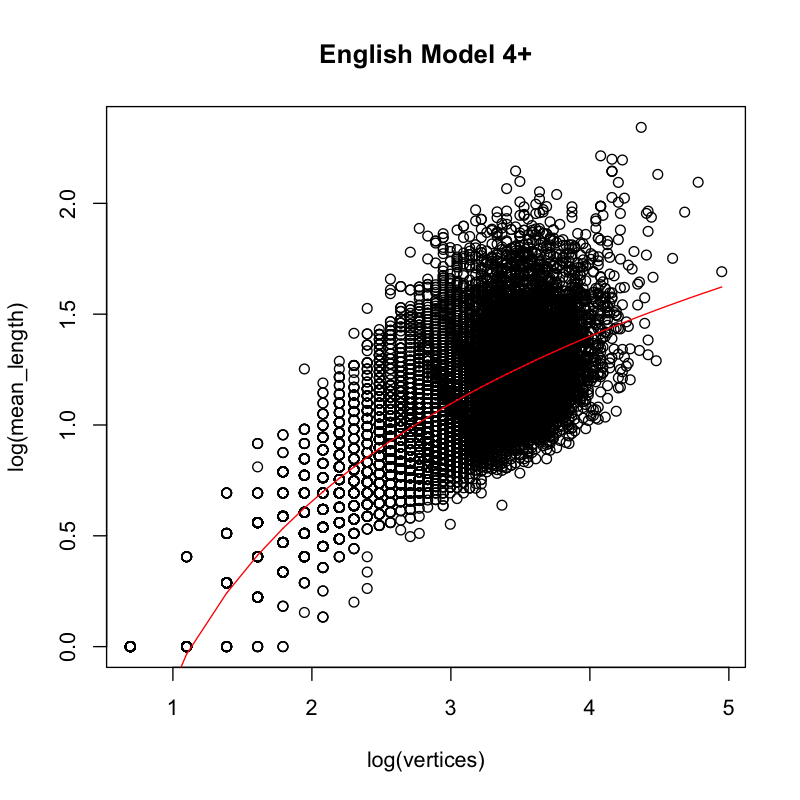
\includegraphics[width=\linewidth]{bestModel_English.png}
  \captionof{figure}{The best model in a log-log plot for English}
  \label{fig:6}
\end{minipage}
\end{figure}

\begin{figure}
\centering
\begin{minipage}{.5\textwidth}
  \centering
  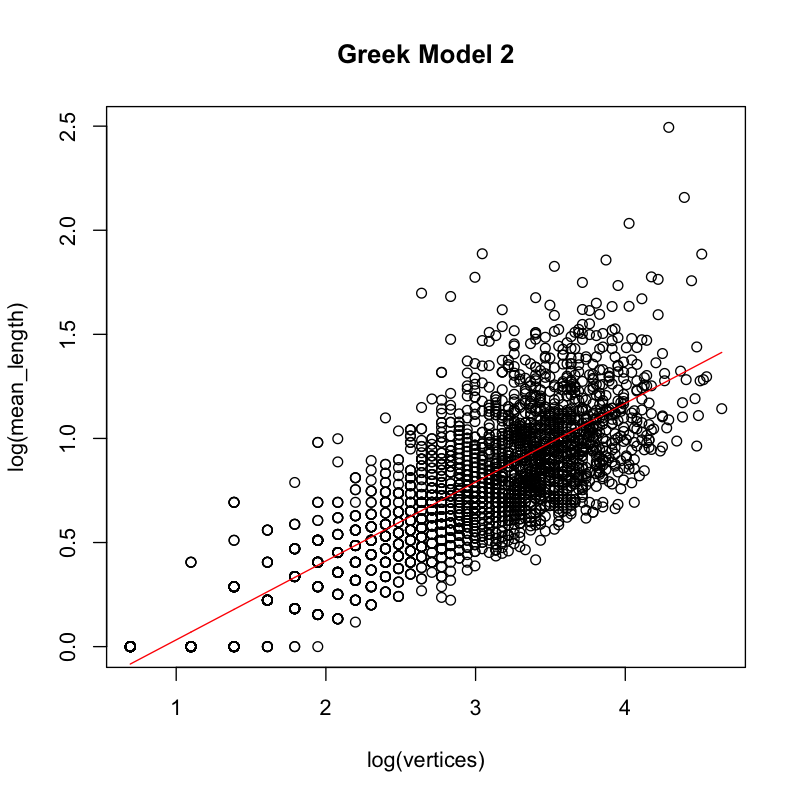
\includegraphics[width=\linewidth]{bestModel_Greek.png}
  \captionof{figure}{The best model in a log-log plot for Greek}
  \label{fig:7}
\end{minipage}%
\begin{minipage}{.5\textwidth}
  \centering
  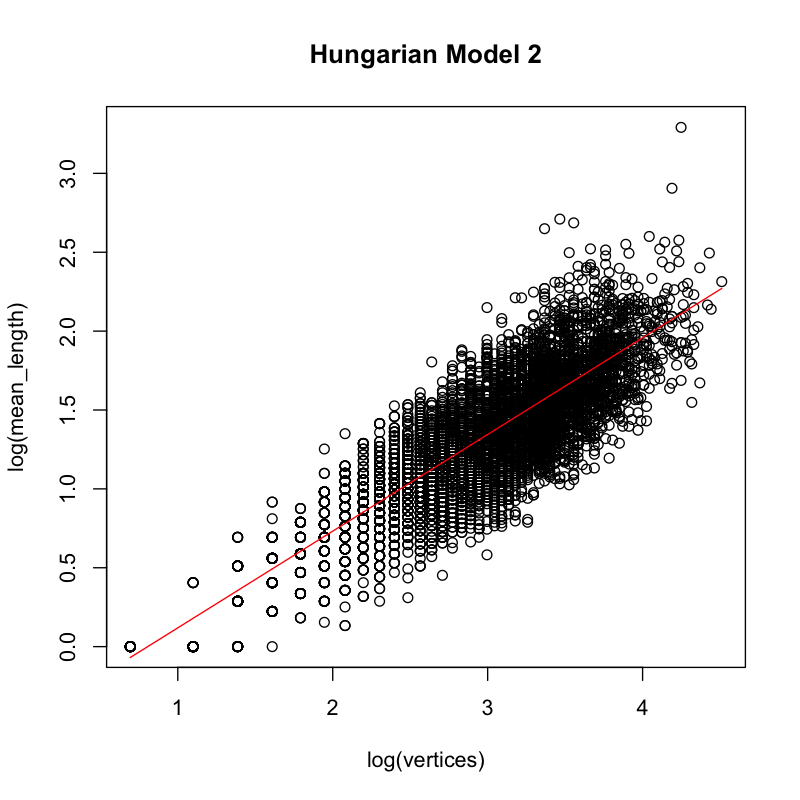
\includegraphics[width=\linewidth]{bestModel_Hungarian.png}
  \captionof{figure}{The best model in a log-log plot for Hungarian}
  \label{fig:8}
\end{minipage}
\end{figure}


\begin{figure}
\centering
\begin{minipage}{.5\textwidth}
  \centering
  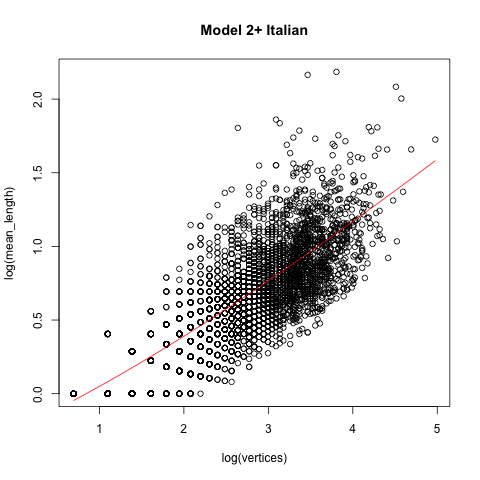
\includegraphics[width=\linewidth]{bestModel_Italian.png}
  \captionof{figure}{The best model in a log-log plot for Italian}
  \label{fig:9}
\end{minipage}%
\begin{minipage}{.5\textwidth}
  \centering
  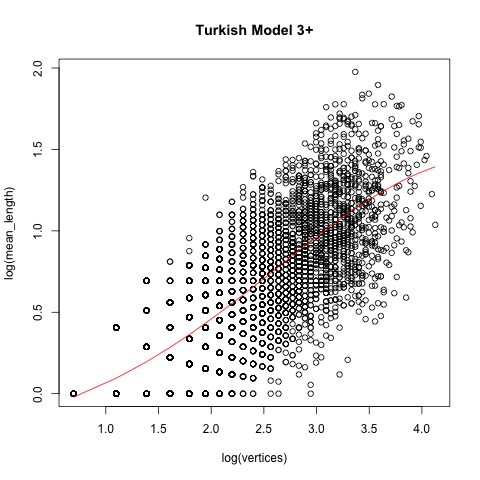
\includegraphics[width=\linewidth]{bestModel_Turkish.png}
  \captionof{figure}{The best model in a log-log plot for Turkish}
  \label{fig:10}
\end{minipage}
\end{figure}

%----------------------------------------------------------------------------------------
%	Comparison aggregated plots
%----------------------------------------------------------------------------------------
\begin{figure}
\centering
\begin{minipage}{\textwidth}
\centering
\begin{minipage}{.5\textwidth}
  \centering
  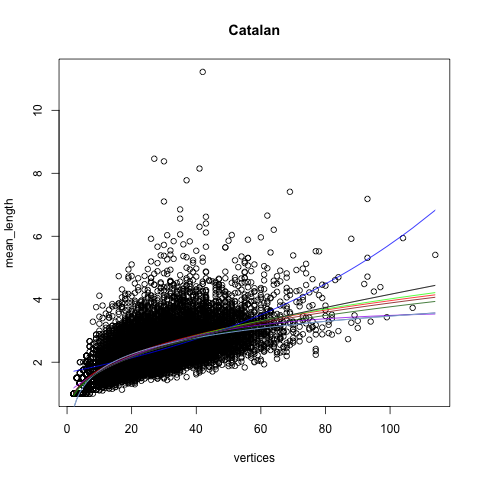
\includegraphics[width=\linewidth]{Mean_Catalan1}
  \captionof*{figure}{Models based on data plotted against data}
  \label{fig:cat1}
\end{minipage}%
\begin{minipage}{.5\textwidth}
  \centering
  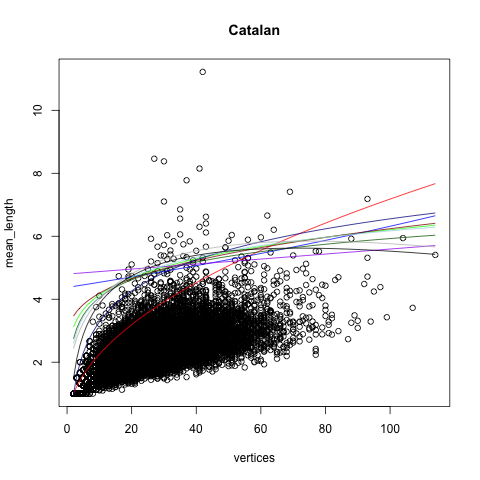
\includegraphics[width=\linewidth]{Mean_Catalan2}
  \captionof*{figure}{Models based on aggregated data plotted against data}
  \label{fig:cat2}
\end{minipage}
\centering
\begin{minipage}{.5\textwidth}
  \centering
  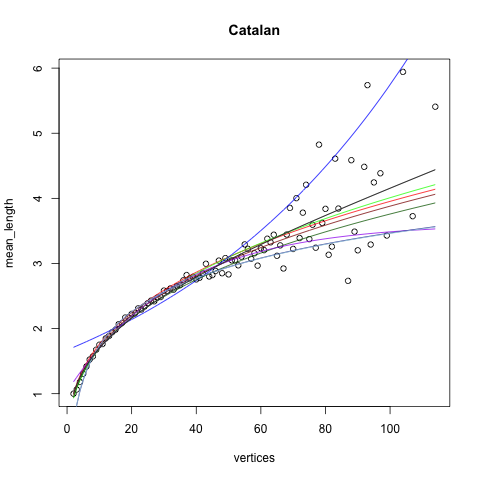
\includegraphics[width=\linewidth]{Mean_Catalan3}
  \captionof*{figure}{Models based on data plotted against aggregated data}
  \label{fig:cat3}
\end{minipage}%
\begin{minipage}{.5\textwidth}
  \centering
  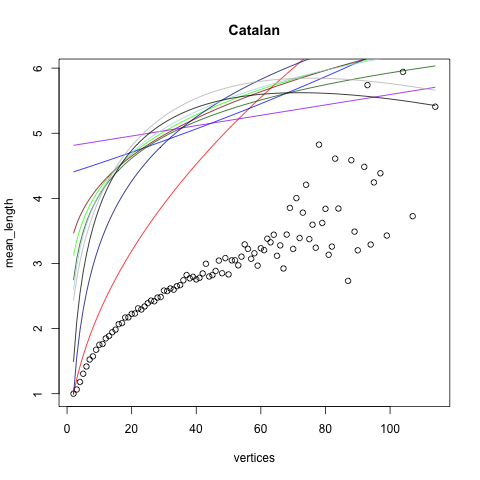
\includegraphics[width=\linewidth]{Mean_Catalan4}
  \captionof*{figure}{Models based on aggregated data plotted against aggregated data}
  \label{fig:cat4}
\end{minipage}
\end{minipage}
\caption{A comparison between the models based on the aggregated data against models based on our original data}\label{fig:compAgg}
\end{figure}


%----------------------------------------------------------------------------------------
%	Discussion
%----------------------------------------------------------------------------------------
\newpage
\section{Discussion}
\subsection{Heteroscedasticity}

\paragraph{Solving Heteroscedasticity}
After we noted that the data was not homoscedastic. We tried aggregating the data and calculating models that data. This didn't turn out well. First we had a lot of trouble with choosing the right starting values (more than when using the original data). And after we succeeded getting a working model it appeared that the approximation was really bad, see plots in Figure~\ref{fig:compAgg}, especially compared to the models on the original data.\\

The aggregated data was hard to approximate, mainly because it consisted of less than $100$ points, which makes it a very sparse dataset. When we looked at the best models for this language, we noted that simpler models were strongly preferred because the RSS was a lot lower and thus the amount of parameters had a higher influence on the AIC.\\

Also the aggregated data gave $1$ weight for every vertex, this means that a vertex with length $5$ will count for as much as a vertex with length $113$, while the first one might have appeared more than $100$ more than the second one. This makes the data very vulnerable for outliers. To solve this, we could add weights when calculating the non-linear model, but we ran out of time to do so.\\

Because of all these problems we decided not to work with the aggregated data, but with the original data.

\subsection{Languages and their best models}
We note in all the plots of the best model that we get a best model that nicely fits the model. In the first image of Figure~\ref{fig:compAgg} we can even see that most models give a reasonably good fit. This is expected, as lots of models resemble each other.

We notice immediately that the best model differs for different languages. For example, the two languages with the lowest $\mu_{n}$ and lowest $\mu_{x}$: Turkish and Chinese both prefer model $3+$. While no other languages prefers this model, nor model $3$.

Depending on the language, also models $1+,2,2+,4+$ and $5$ get selected as a model. 

We also noticed that, for most languages (except Catalan, Chinese and Turkish) model $5$ is very close to the best result.

\subsection{Conclusions}
So we can conclude that a combination of model $5$ and model $3+$ would lead to good best fits for all models. We also note that probably model $5+$ alone would be sufficient as well, but then we would have to tune the starting values a lot better and solve some extra issues.\\

We can also conclude that for some languages the model for the mean length of the edges of the dependency tree as a function of the number of words significantly differs from the models for other languages.\\

To finish we found that we have found a model with a good fit for every language.

%----------------------------------------------------------------------------------------
%	Methods
%----------------------------------------------------------------------------------------
\section{Methods}
We employed several methods for finding starting values. If there was no additive term, a linear approximation was usually sufficient. When there was an additive term, this usually wasn't. So we mainly did some manual search, using the expand.grid and nls2 functions. Once a starting value was found, it usually worked for a lot of languages.\\
When evaluating the mean data, we could evaluate a grid every time before starting, to get better results.\\
To automate the process, we used selfstarters.\\

After we find good starting values for the original data for almost every language and model, a few errors remained. To solve these, we adapted the maximum iterations for the model and also the tolerance and the minFactor. At last we set warnOnly True, so that we could fully automate the calculation of the best model and didn't have to worry about these errors. Running all models for all languages we get $2$ errors (for model 5+) and we consider this acceptable.

\end{document}